\newpage


\section{Analisi}
\label{sec:analisi}
In questa sezione verrà effettuata un'analisi sui risultati mediati su 30 simulazioni, 
comparando il modello base con il modello esteso e infine con un modello allo stato dell'arte.

\subsection{Modello Base}
Nelle figure \ref{fig:analisi-base-evacuated} e \ref{fig:analisi-base-casualties} vengono mostrate le percentuali di evacuati 
e di morti nel tempo, al variare del numero di auto e pedoni.
%
Come si può notare dalla figura \ref{fig:analisi-base-evacuated}, il numero di pedoni non influenza la percentuale di pedoni evacuati nel tempo.
%
Per quanto riguarda le auto, più è alto il numero di auto più tempo è richiesto per evacuare e inoltre più bassa è la percentuale di auto evacuate alla fine della simulazione.
%
% TODO: rivedere
Osservando le evacuazioni totali invece risulta che la configurazione che permette di evacuare più agenti sia la 50\% - 50\%, mentre la configurazione 0\% - 100\% sia la peggiore.

\begin{figure}[ht]
    \centering
    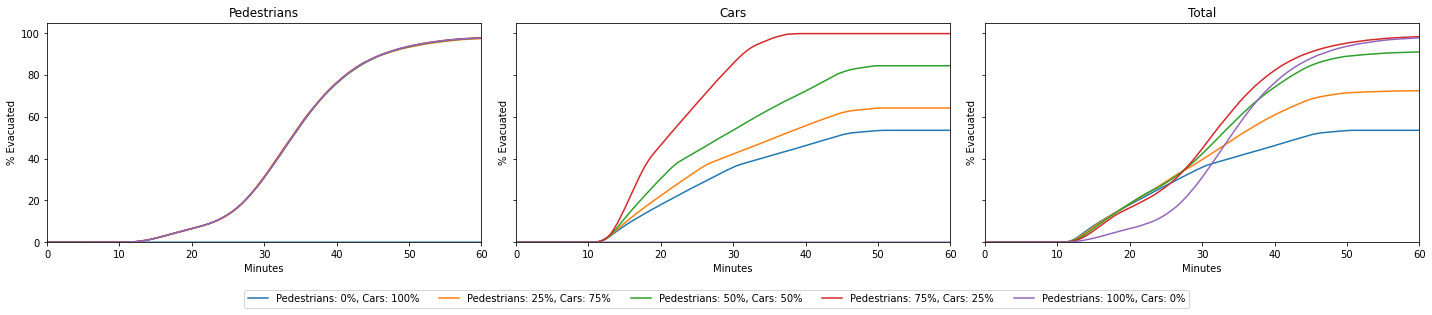
\includegraphics[width=\textwidth]{images/analisi/base-evacuated.png}
    \caption{Percentuale degli evacuati nel tempo al variare del numero di agenti con il modello base.}
    \label{fig:analisi-base-evacuated}
\end{figure}

Per quanto riguarda le percentuali di mortalità (Fig. \ref{fig:analisi-base-casualties}), per i pedoni rimangono sotto al 2\% in tutti i casi.
%
Per le auto invece nei casi con una percentuale di auto di 25\% e 50\% non c'é nessuna vittima, mentre 
con una percentuale di 75\% si ha una mortalità di 1.8\% e nel caso peggiore, ovvero 100\%, si raggiunge circa il 10\% di vittime.
%
Infine osservando le morti totali risulta che il caso migliore sia uno scenario bilanciato tra auto e pedoni, 
mentre i casi con una mortalità maggiore siano quelli con solo pedoni o solo auto.

\begin{figure}[ht]
    \centering
    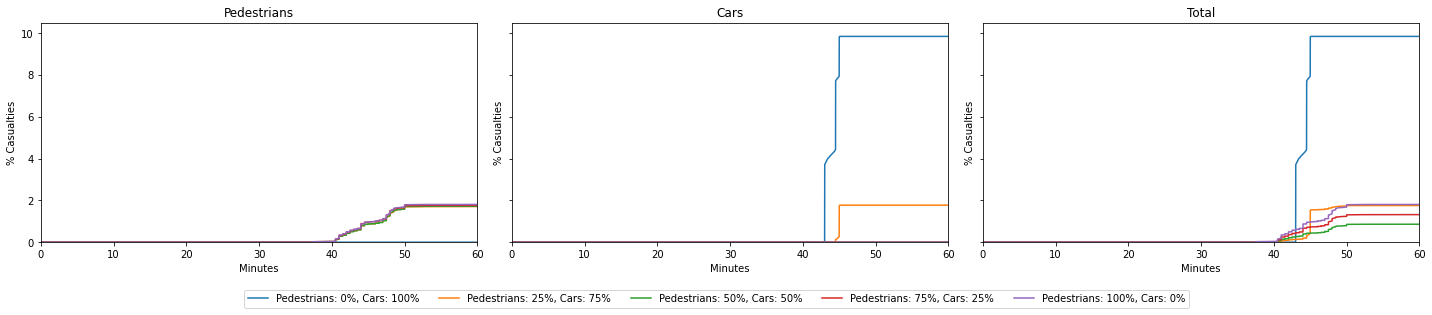
\includegraphics[width=\textwidth]{images/analisi/base-casualties.png}
    \caption{Percentuale delle vittime nel tempo al variare del numero di agenti con il modello base.}
    \label{fig:analisi-base-casualties}
\end{figure}

Nella figura \ref{fig:analisi-base-evtimes} vengono riportate le distribuzioni delle percentuali di agenti evacuati ad ogni minuto della simulazione.
%
% TODO: sistemare
Si può osservare come all'aumentare del numero di auto considerate in una simulazione la media tenda a spostarsi verso sinistra.
In particolare nel caso 50\%-50\% due picchi sembrano formarsi un molto probabilmente per le auto 
il primo mentre il secondo per i pedoni, quest'ultimo tende ad appiattirsi con il crescere del 
numero di auto fino a sparire nel caso 0\%-100\%.

\begin{figure}[ht]
    \centering
    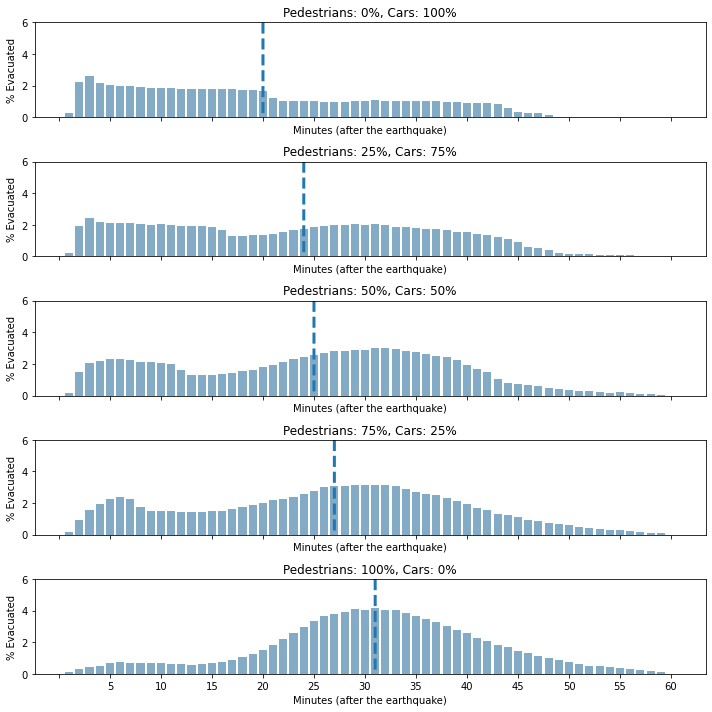
\includegraphics[width=\textwidth]{images/analisi/base-evtimes.png}
    \caption{Distribuzione del tempo di evacuzione in percentuale al variare del numero di agenti con il modello base.}
    \label{fig:analisi-base-evtimes}
\end{figure}

\pagebreak

\subsection{Modello Esteso}
Nonostante l'introduzione della variazione della velocità per i pedoni, 
la percentuale di pedoni evacuati risulta molto simile al variare del numero di pedoni (Fig. \ref{fig:analisi-new-evacuated}). 
Si può notare una differenza significativa tra il minuto 30 e il minuto 40 per il caso 100\% pedoni.

In generale il numero di auto evacuate é molto più basso rispetto a quello dei pedoni. 
Il caso con una percentuale di auto evacuate maggiore è quello con il 25\% di auto e il 75\% di pedoni.
Il caso con solo auto, al contrario di come si possa pensare, non é il caso peggiore e ha un numero di evacuati simile ai casi 
con 75\% e 50\% di auto.
%
In tutti i casi le auto evacuano prima dei pedoni avendo una velocità superiore.

Considerando i contributi di auto e pedoni, al diminuire del numero di auto considerate cresce il numero totale di evacuati alla fine della simulazione,
fino al caso migliore con solo pedoni.

\begin{figure}[ht]
    \centering
    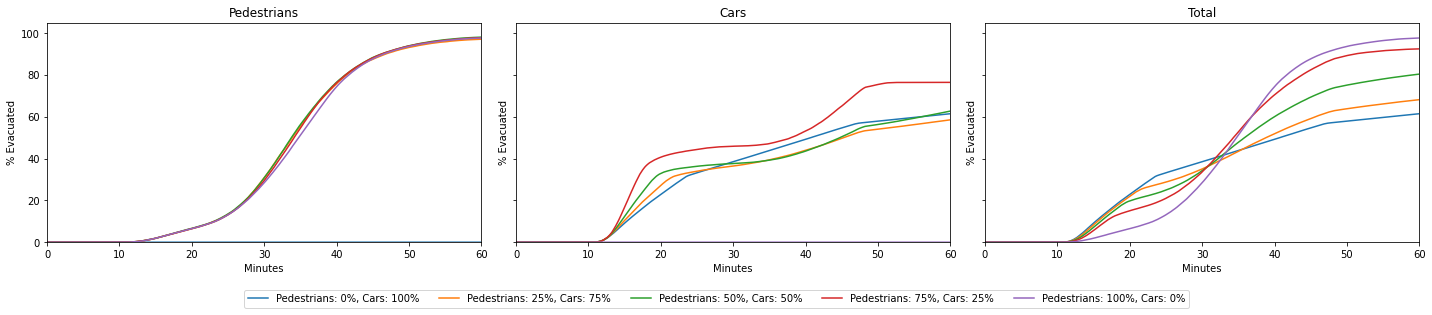
\includegraphics[width=\textwidth]{images/analisi/new-evacuated.png}
    \caption{Percentuale degli evacuati nel tempo al variare del numero di agenti con il modello esteso.}
    \label{fig:analisi-new-evacuated}
\end{figure}

Nella figura \ref{fig:analisi-new-casualties} si può vedere come al variare del numero di pedoni considerati 
non ci siano differenze significative, mentre per le auto il numero di vittime sale al crescere del numero di auto considerate.
In generale la percentuale di vittime per le auto è molto più alto rispetto a quello dei pedoni, con un massimo di circa 37\% nel caso con 75\% di auto. 
%
Il numero di vittime totali cresce al crescere del numero di auto.

\begin{figure}[ht]
    \centering
    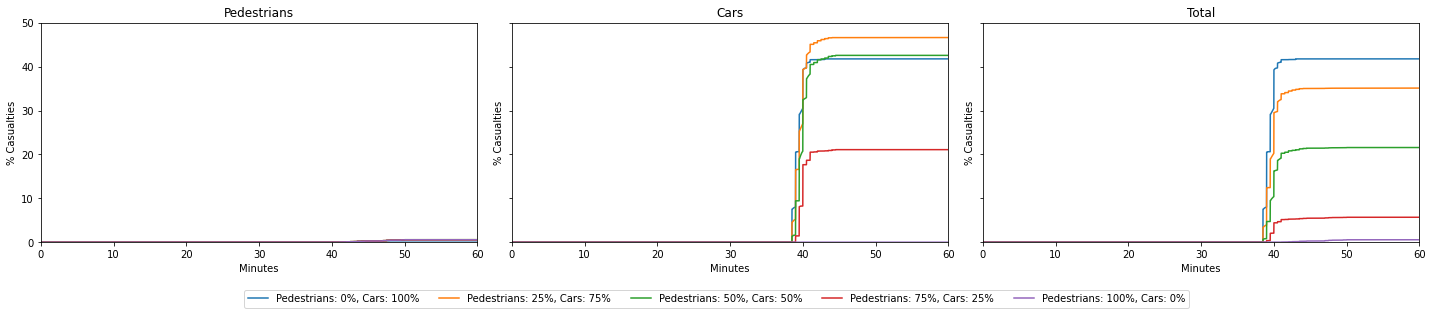
\includegraphics[width=\textwidth]{images/analisi/new-casualties.png}
    \caption{Percentuale delle vittime nel tempo al variare del numero di agenti con il modello esteso.}
    \label{fig:analisi-new-casualties}
\end{figure}

\pagebreak

La distribuzione della percentuale di evacuati nel tempo \ref*{fig:analisi-new-evtimes} ha un comportamento analogo a quello del modello base, con un aumento del tempo medio di evacuazione.

\begin{figure}[ht]
    \centering
    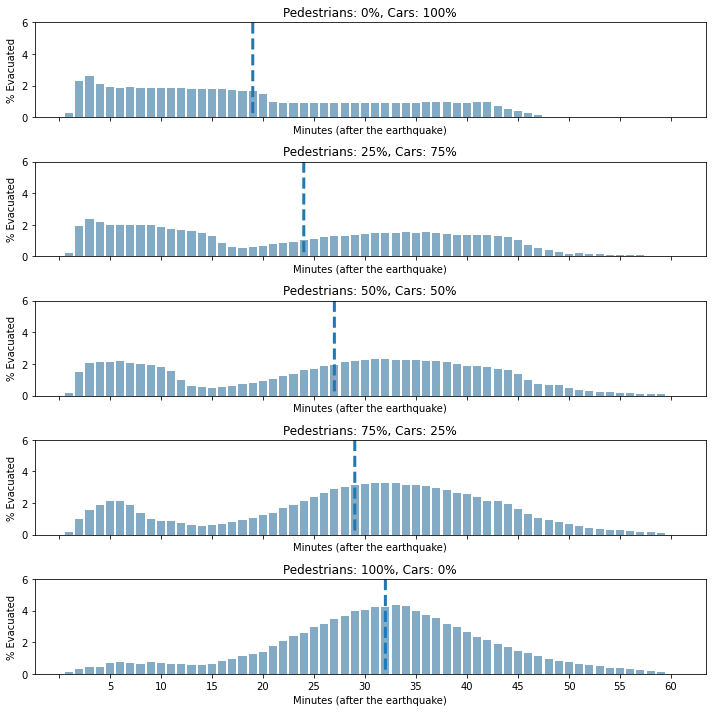
\includegraphics[width=\textwidth]{images/analisi/new-evtimes.png}
    \caption{Distribuzione del tempo di evacuzione in percentuale al variare del numero di agenti con il modello esteso.}
    \label{fig:analisi-new-evtimes}
\end{figure}

\subsection{Comparazione Modello Base e Modello Esteso}
% TODO: sistemare
In questa sottosezione verrano comparati il modello base con il modello esteso analizzando,
le percentuali di evacuati e di morti nel tempo al variare del numero di auto e pedoni per poi passare a comparazioni spaziali,
in particolare mostrando l'efficienza delle intersezioni e l'effetto causato durante la simulazione.

\pagebreak
\subsubsection*{Percentuale di vittime ed evacuati}

\begin{figure}[ht]
    \centering
    \begin{subfigure}{0.45\textwidth}
        \centering
        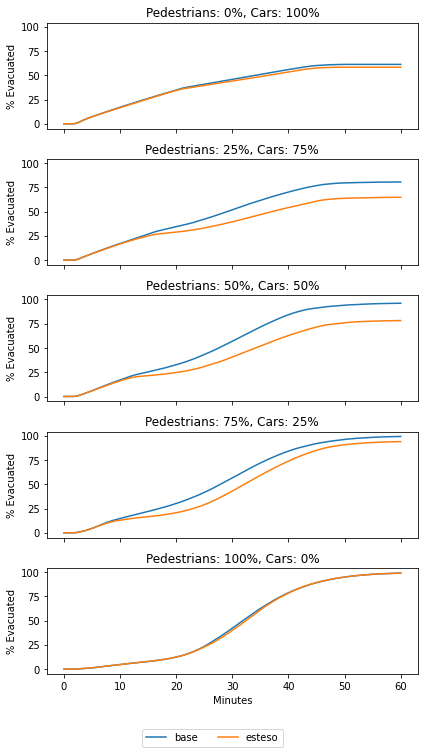
\includegraphics[width=\textwidth]{images/analisi/comparison-total-evacuated.png}
    \end{subfigure}
    \hfill
    \begin{subfigure}{0.45\textwidth}
        \centering
        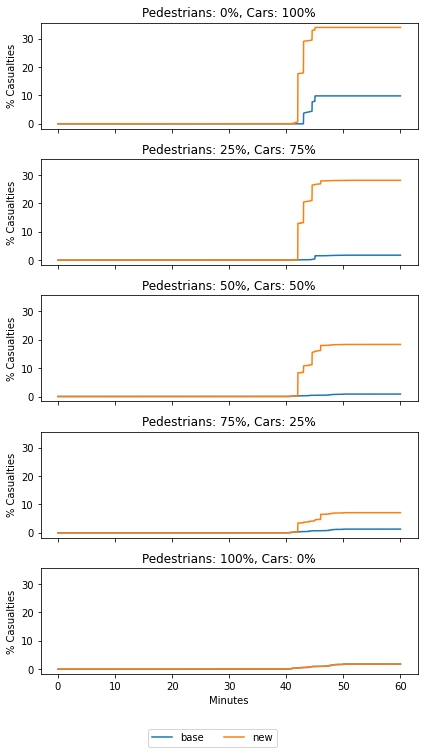
\includegraphics[width=\textwidth]{images/analisi/comparison-total-casualties.png}
    \end{subfigure}
    \caption{Comparazione tra modello base e modello esteso delle percentuali di agenti evacuati (sinistra) e di agenti morti (destra) al variare del numero di agenti.}
    \label{fig:analisi-comparison-total-ec}
\end{figure}

\newpage

Osservando la figura \ref{fig:analisi-comparison-total-ec} è possibile comparare le percentuali di evacuati e morti a diversi split tra i due modelli.
In generale il modello esteso presenta un numero minore di evacuati e un numero maggiore di vittime rispetto al modello base.
Per entrambi i modelli la percentuale di evacuati decresce all'aumentare del numero di auto considerate, mentre la percentuale di vittime cresce.
Inoltre per entrambi i modelli le prime vittime si verificano dopo 40 min.

gli unici casi in cui il modello esteso si avvicina ai risultati del modello base sono il caso con solo pedoni ed il caso 75\%-25\%.

\subsubsection*{Distribuzione dei tempi di evacuazione}

Come già detto in precedenza le distribuzioni di percentuale di evacuati nel tempo \ref{fig:analisi-comparison-evtimes} del modello base e del modello esteso 
presentano un andamento simile con un aumento del tempo medio di evacuazione.


\begin{figure}[ht]
    \centering
    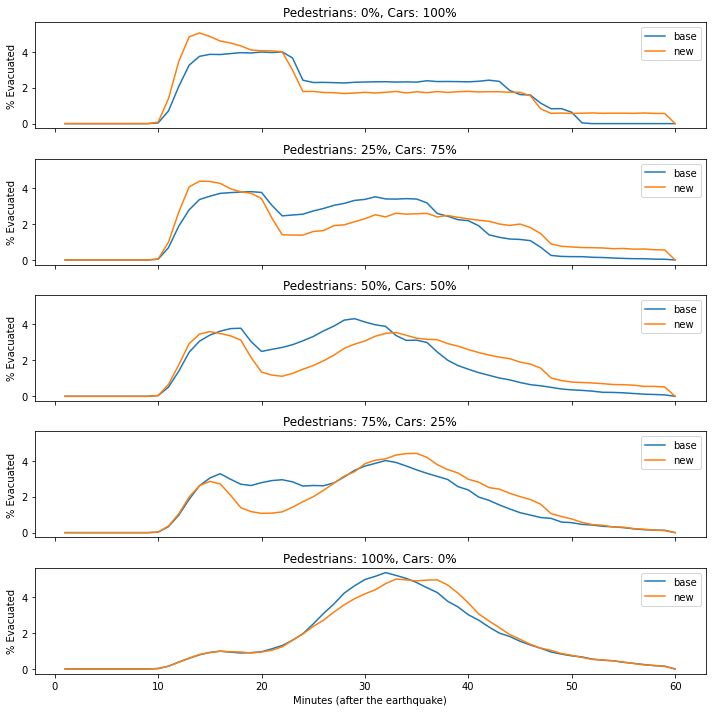
\includegraphics[width=0.9\textwidth]{images/analisi/comparison-evtimes.png}
    \caption{Comparazione delle distribuzioni dei tempi di evacuazione al variare del numero di agenti.}
    \label{fig:analisi-comparison-evtimes}
\end{figure}


\begin{figure}[ht]
    \centering
    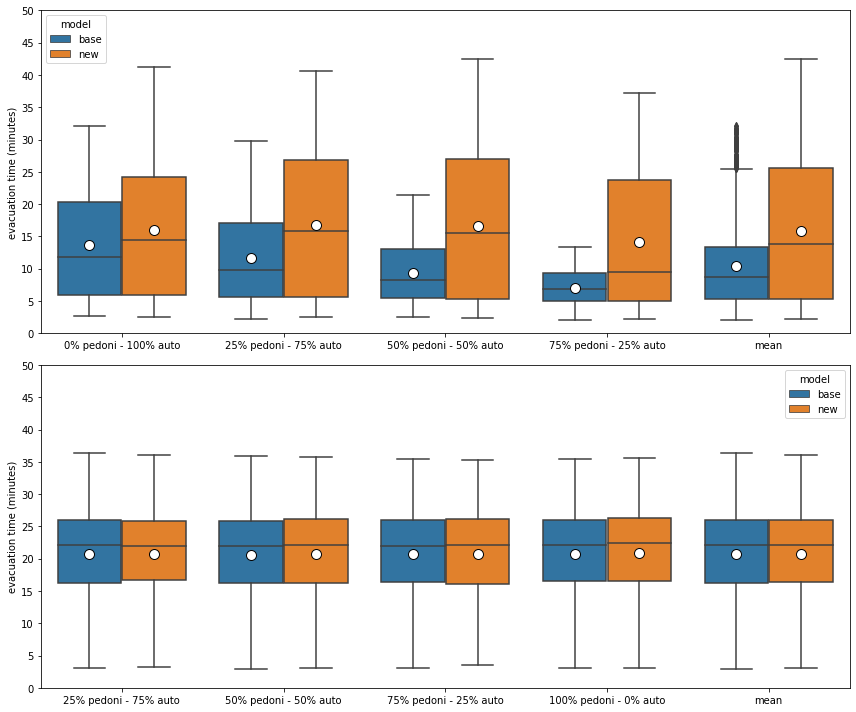
\includegraphics[width=0.9\textwidth]{images/analisi/comparison-evtimes2.png}
    \caption{
        Comparazione dei tempi di evacuazione al variare del numero di agenti e nel caso medio distinti per auto (sopra) e pedoni (sotto).
    }
    \label{fig:analisi-comparison-evtimes2}
\end{figure}

Nella figura \ref{fig:analisi-comparison-evtimes2} vengono confrontati i tempi di evacuazione tra auto e pedoni.
Per quanto riguarda le auto, il modello base presenta un andamento descresente per il tempo medio richiesto per evacuare al diminuire del numero di auto considerate.
Le auto impiegano in media tempi maggiori con il modello esteso rispetto a quello base.
%
I pedoni invece non presentano alcun cambiamento significativo al variare del numero di agenti e del modello considerato. 

Per entrambi i modelli un pedone impiega in media un tempo di 21 minuti per evacuare e un massimo di 36 minuti.
Per le auto invece il tempo medio di evacuazione per il modello base è 10 minuti e per il modello esteso 16 minuti, 
con tempi massimi rispettivamente di 32 e 42 minuti.

\pagebreak

La figura \ref{fig:analisi-comparison-ev-times-map} mostra i tempi di evacuazione mediati tra gli agenti che partono dalla stessa intersezione,
mediati a loro volta tra tutte le configurazioni di auto e pedoni.

In generale gli agenti che partono dalla costa impiegano più tempo rispetto agli altri che sono più vicini ai rifugi.

Confrontando i pedoni al variare del modello usato non si riscontrano cambiamenti significativi nei tempi di evacuazione (\ref{fig:2d-evtimes-base-ped}, \ref{fig:2d-evtimes-new-ped}).
Mentre nel caso delle auto si nota che il modello esteso introduca dei rallentamenti rispetto al modello base, soprattuto lungo la costa (\ref{fig:2d-evtimes-base-car}, \ref{fig:2d-evtimes-new-car}).


\begin{figure}[ht]
    \centering
    \begin{subfigure}{0.475\textwidth}
        \centering
        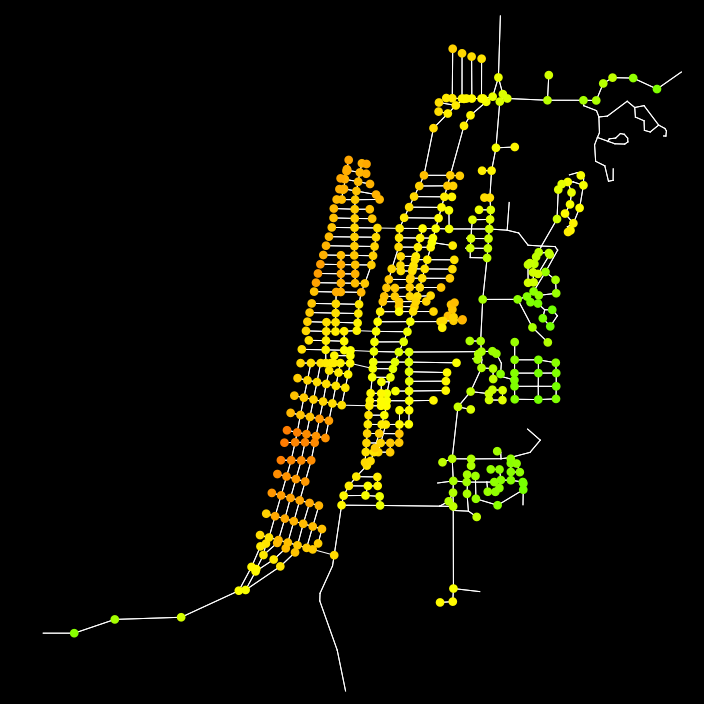
\includegraphics[width=\textwidth]{images/analisi/comparison-ev-times-map-base-ped.png}
        \caption{Pedoni nel modello base}
        \label{fig:2d-evtimes-base-ped}
    \end{subfigure}
    \hfill
    \begin{subfigure}{0.475\textwidth}
        \centering
        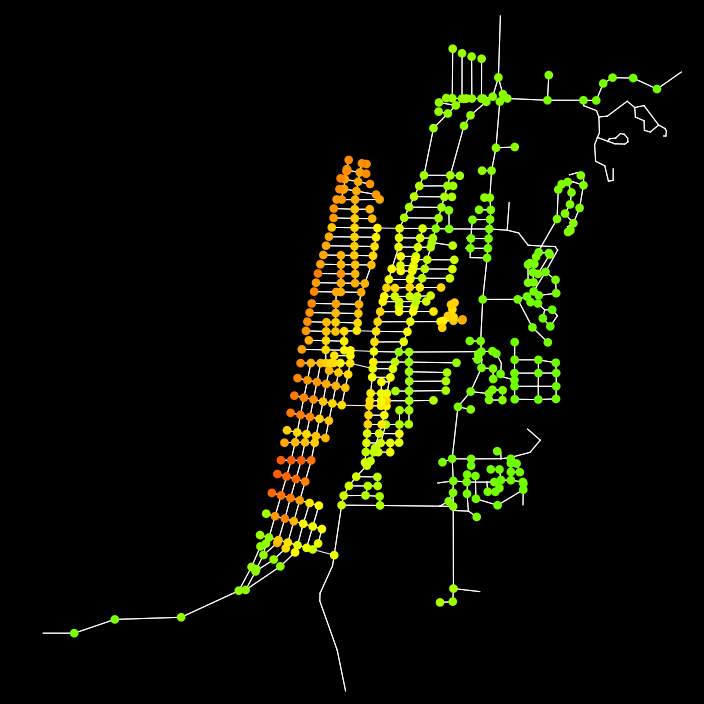
\includegraphics[width=\textwidth]{images/analisi/comparison-ev-times-map-new-ped.png}
        \caption{Pedoni nel modello esteso}
        \label{fig:2d-evtimes-new-ped}
    \end{subfigure}
    \hfill
    \begin{subfigure}{0.475\textwidth}
        \centering
        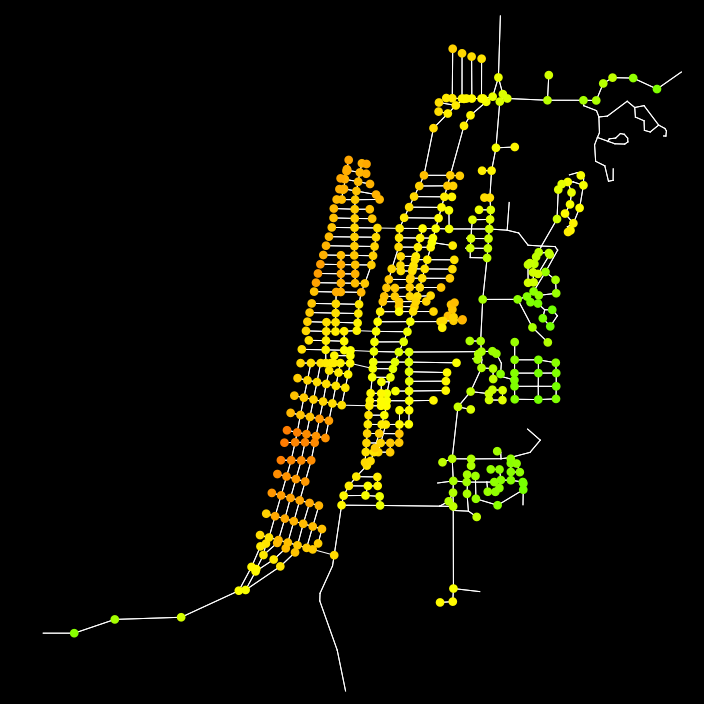
\includegraphics[width=\textwidth]{images/analisi/comparison-ev-times-map-base-car.png}
        \caption{Auto nel modello base}
        \label{fig:2d-evtimes-base-car}
    \end{subfigure}
    \hfill
    \begin{subfigure}{0.475\textwidth}
        \centering
        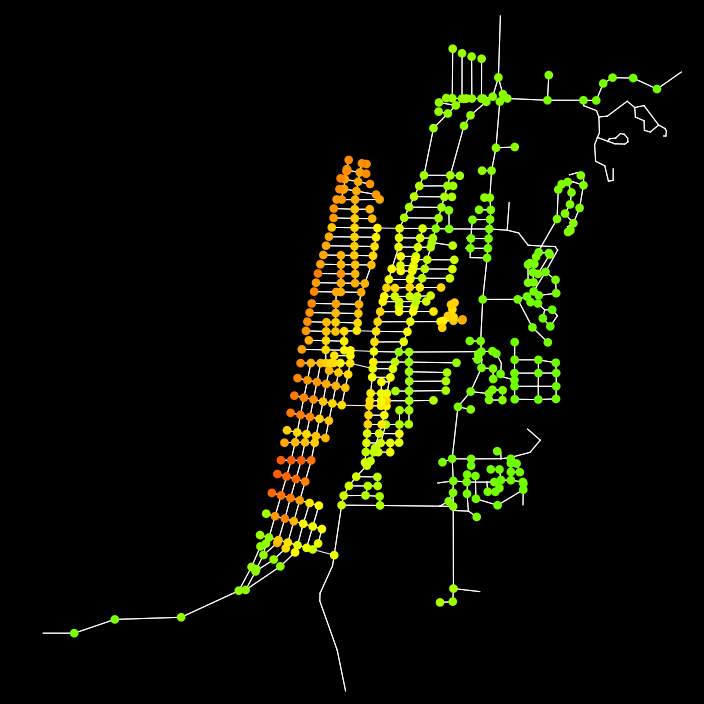
\includegraphics[width=\textwidth]{images/analisi/comparison-ev-times-map-new-car.png}
        \caption{Auto nel modello esteso}
        \label{fig:2d-evtimes-new-car}
    \end{subfigure}
    \caption{Comparazione dei tempi di evacuazione mediati tra gli agenti che partono dalla stessa intersezione. }
    \label{fig:analisi-comparison-ev-times-map}
\end{figure}

\subsubsection*{Strade Critiche}

Un'ulteriore analisi per valutare l'effetto dell'estensione del modello è quella di evidenziare in quali strade si verificano 
più vittime al variare del numero di auto e pedoni. 

Nella figura \ref{fig:analisi-comparison-critical-links1} viene mostrato come si distribusce la percentuale di mortalità nelle strade 
al variare del numero di auto e pedoni e riportata la percentuale media. 

Il modello base (Fig. \ref{fig:base-link-casualties}) nei casi con un numero di auto minore o uguale al 50\%
non presenta differenze significative e si hanno tante strade con una percentuale bassa di vittime, 
mentre negli altri due casi ci sono poche strade con una percentuale alta.

Il modello esteso (Fig. \ref{fig:new-link-casualties}) invece presenta una strada comune per tutti casi 
in cui sono presenti delle auto che contribuisce a più del 50\% delle vittime.

In generale in tutti i casi la maggior parte delle strade con più vittime sono diverse tra i due modelli a eccezione del caso 
100\% pedoni.

Le strade segnate come critiche corrispondono a quelle con una percentuale media maggiore del 5\% e sono mostrate nella figura \ref{fig:analisi-comparison-critical-links2}.

\begin{figure}[ht]
    \centering
    \begin{subfigure}{0.475\textwidth}
        \centering
        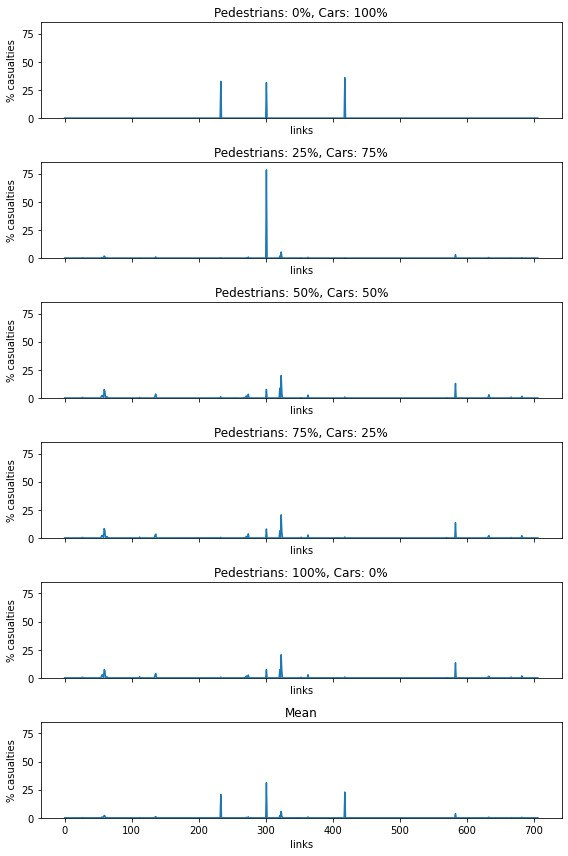
\includegraphics[width=\textwidth]{images/analisi/base_links_casualties}
        \caption{Modello base}
        \label{fig:base-link-casualties}
    \end{subfigure}
    \hfill
    \begin{subfigure}{0.475\textwidth}
        \centering
        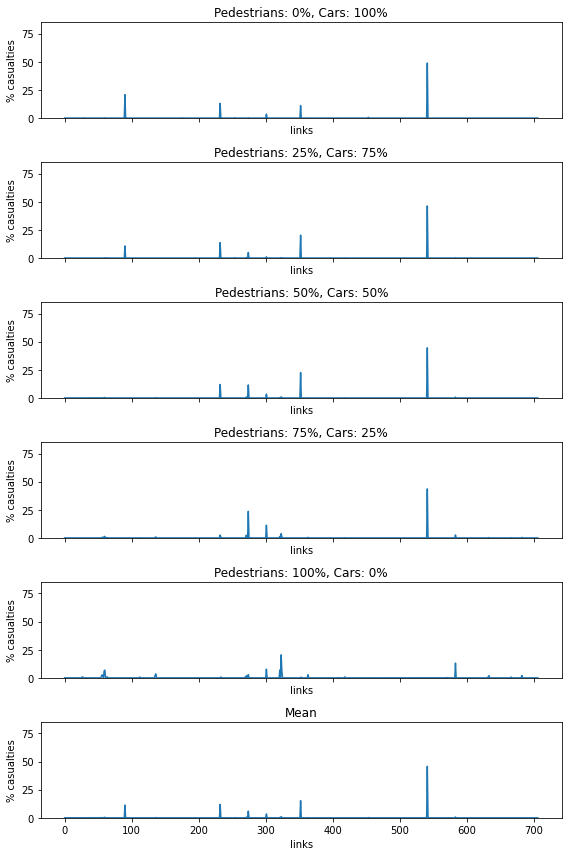
\includegraphics[width=\textwidth]{images/analisi/new_links_casualties}
        \caption{Modello esteso}
        \label{fig:new-link-casualties}
    \end{subfigure}
    \caption{Comparazione delle percentuali di mortalità nelle strade al variare del numero di auto e pedoni.}
    \label{fig:analisi-comparison-critical-links1}
\end{figure}

\begin{figure}[ht]
    \centering
    \begin{subfigure}{0.475\textwidth}
        \centering
        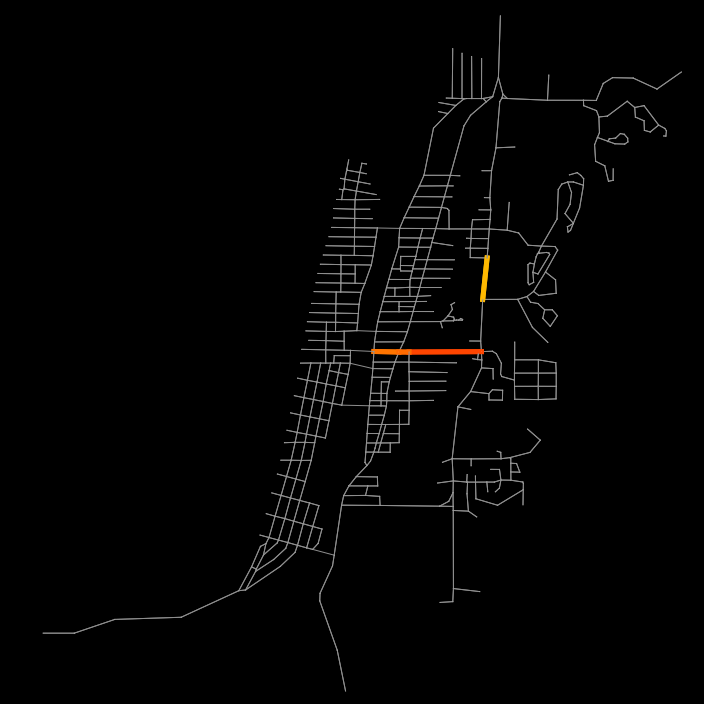
\includegraphics[width=\textwidth]{images/analisi/comparison-base-critical-links.png}
        \caption{Modello base}
    \end{subfigure}
    \hfill
    \begin{subfigure}{0.475\textwidth}
        \centering
        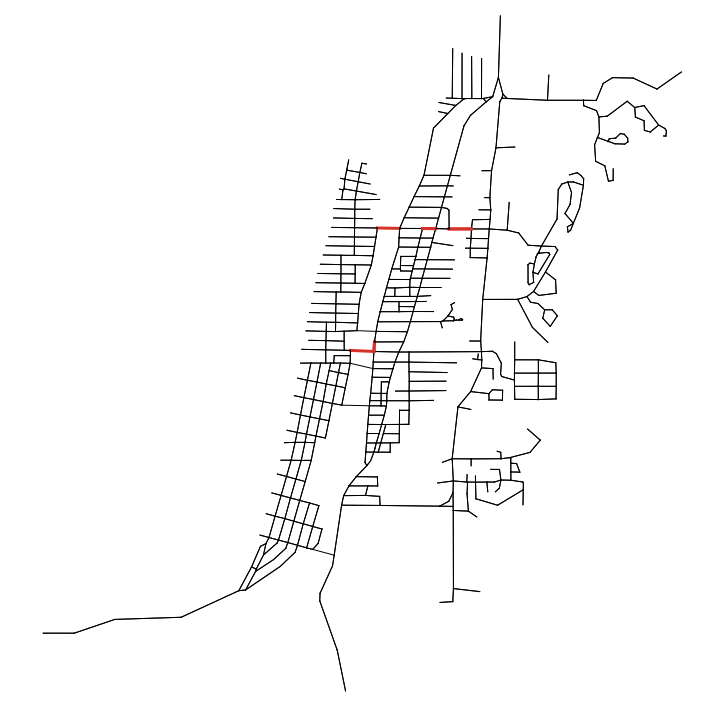
\includegraphics[width=\textwidth]{images/analisi/comparison-new-critical-links.png}
        \caption{Modello esteso}
    \end{subfigure}
    \caption{Strade critiche trovate per i due modelli.}
    \label{fig:analisi-comparison-critical-links2}
\end{figure}

\subsubsection*{Flusso}
Delle ulteriori analisi sono state effettuate per le intersezioni. Sono stati confrontati i 
flussi in entrata e in uscita e i tempi di attesa delle intersezioni per i due modelli 
al variare del numero di auto e di pedoni.

%
% TODO: rivedere
Come si nota nella figura \ref{fig:analisi-comparison-in-out-flow-ped}, il flusso dei pedoni
in entrambi i modelli risulta abbastanza bilanciato,
infatti i punti formati dalle coppie di flusso in entrata e di flusso in uscita si distribuiscono su una retta.
L'unica differenza che si nota è l'incremento del flusso all'aumentare del numero dei pedoni,
mentre non si notano grosse differenze tra i due modelli e nemmeno tra i due tipi di incrocio.


\begin{figure}[ht]
    \centering
    \begin{subfigure}{0.99\textwidth}
        \centering
        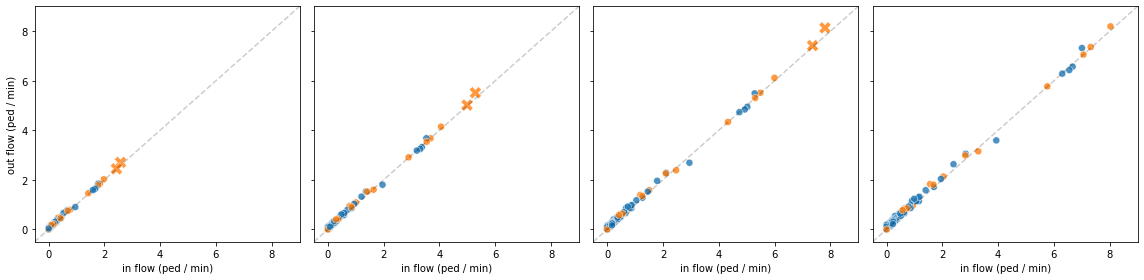
\includegraphics[width=\textwidth]{images/analisi/comparison-base-in-out-flow-ped.png}
        \caption{Modello base}
    \end{subfigure}
    \begin{subfigure}{0.99\textwidth}
        \centering
        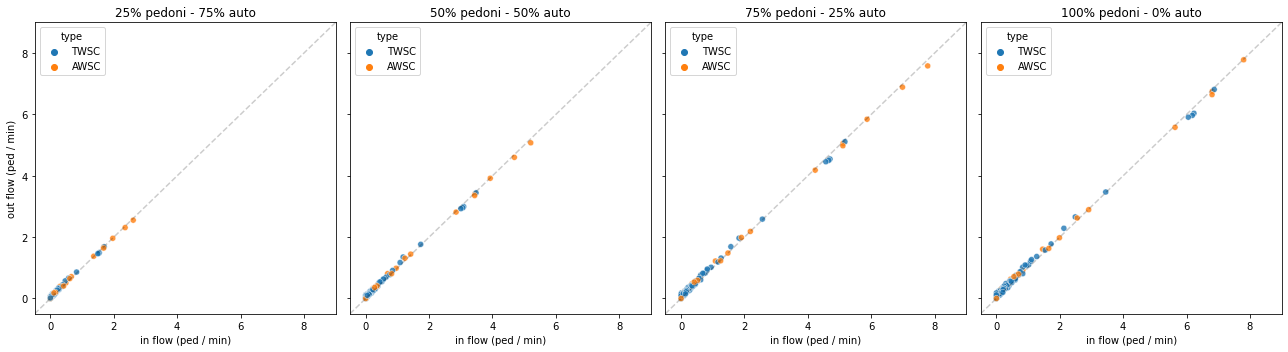
\includegraphics[width=\textwidth]{images/analisi/comparison-new-in-out-flow-ped.png}
        \caption{Modello esteso}
    \end{subfigure}
    \caption{
        Confronto tra il flusso dei pedoni in entrata e in uscita per ogni intersezione al variare del numero di auto e pedoni.
    }
    \label{fig:analisi-comparison-in-out-flow-ped}
\end{figure}
% TODO: rivedere
Osservando il flusso delle auto (Fig. \ref{fig:analisi-comparison-in-out-flow-car}), anche in questo caso
non si notano grosse differenze tra AWSC e TWSC e viene sempre riscontrato un incremento di flusso all'aumentare del numero di auto.
In questo caso però il flusso in entrata e in uscita non sono perfettamente bilanciati discostandosi dal formare una retta ideale.
infatti il flusso in entrata è quasi sempre maggiore del flusso in uscita.
La differenza che più si nota tra il modello esteso ed il modello base è un abbassamento sostanziale del flusso,
molto probabilmente dovuto alla gestione delle intersezioni.
Infine le intersezioni più critiche vengono evidenziate spazialmente sia per il modello base 
(Fig. \ref{fig:analisi-comparison-in-out-flow-map-base}) che per il modello esteso (Fig. \ref{fig:analisi-comparison-in-out-flow-map-new}).
Gli incroci più critici sono identificati dai punti che superano una distanza di 3 dalla retta y = x,
si può notare come il numero di incroci critici aumenti con il numero di auto.

\begin{figure}[ht]
    \centering
    \begin{subfigure}{0.99\textwidth}
        \centering
        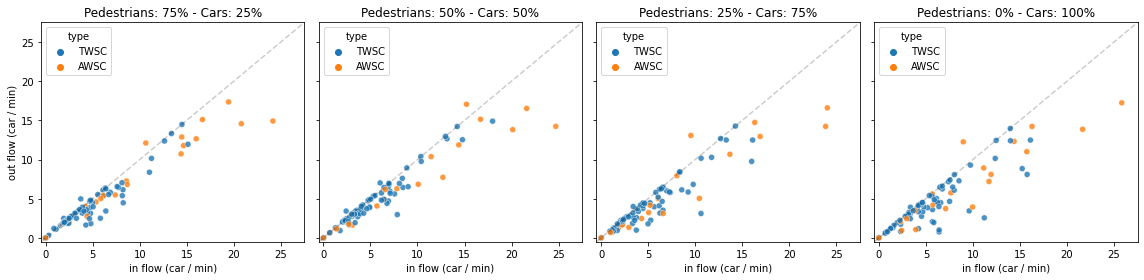
\includegraphics[width=\textwidth]{images/analisi/comparison-base-in-out-flow-car.png}
        \caption{Modello base}
    \end{subfigure}
    \begin{subfigure}{0.99\textwidth}
        \centering
        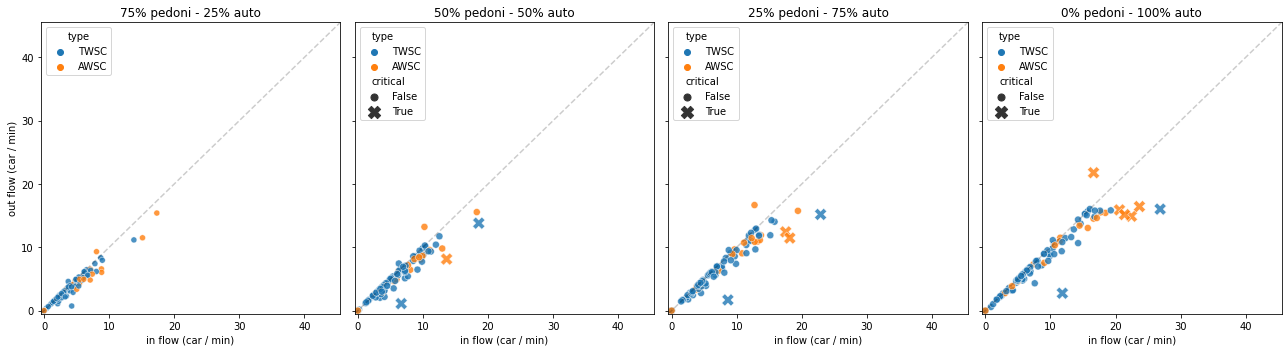
\includegraphics[width=\textwidth]{images/analisi/comparison-new-in-out-flow-car.png}
        \caption{Modello estenso}
    \end{subfigure}
    \caption{
        Confronto tra il flusso delle auto in entrata e in uscita per ogni intersezione al variare del numero di auto e pedoni.
        I punti che hanno una distanza maggiore o uguale a 3 dalla retta sono marcati come critici.
    }
    \label{fig:analisi-comparison-in-out-flow-car}
\end{figure}

\begin{figure}[ht]
    \centering
    \begin{subfigure}{0.475\textwidth}
        \centering
        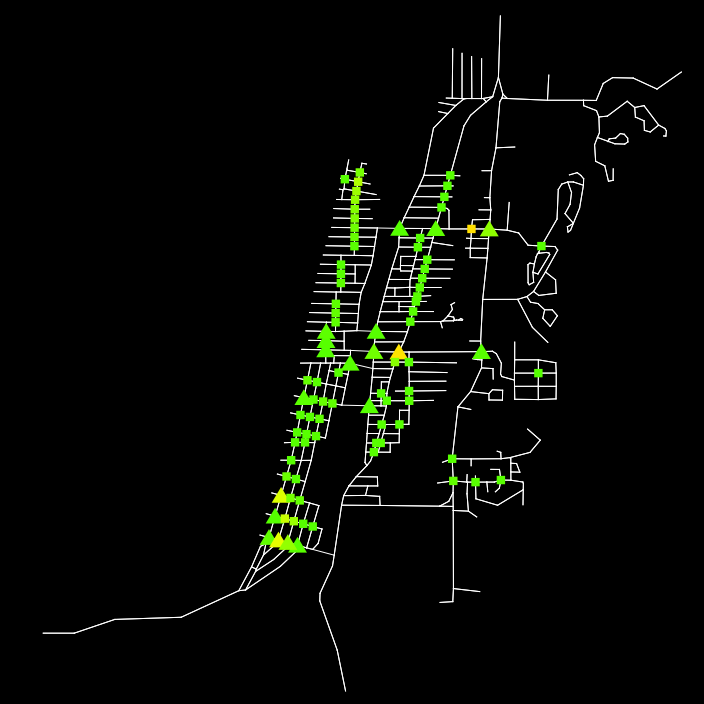
\includegraphics[width=\textwidth]{images/analisi/comparison-base-in-out-flow-75-25-car.png}
        \caption{75 pedoni 25 auto}
    \end{subfigure}
    \begin{subfigure}{0.475\textwidth}
        \centering
        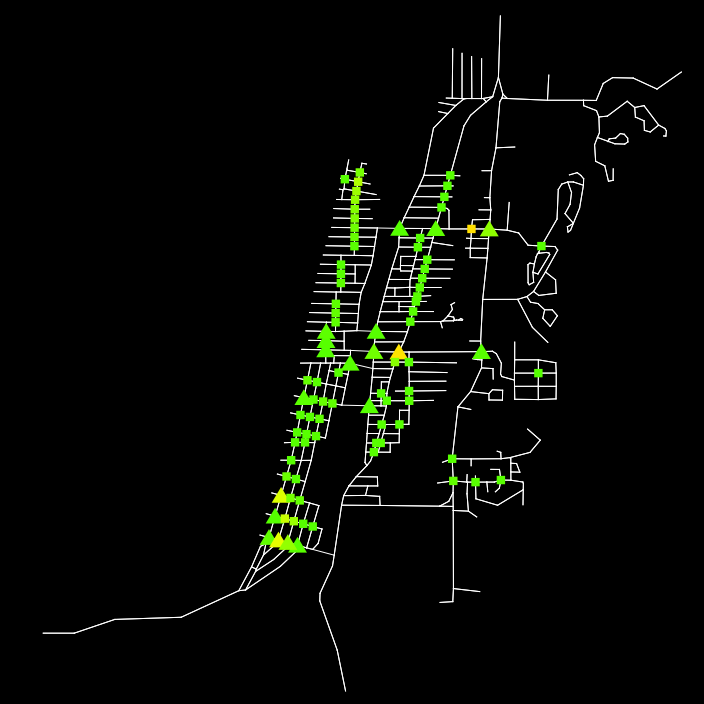
\includegraphics[width=\textwidth]{images/analisi/comparison-base-in-out-flow-50-50-car.png}
        \caption{50 pedoni 50 auto}
    \end{subfigure}
    \begin{subfigure}{0.475\textwidth}
        \centering
        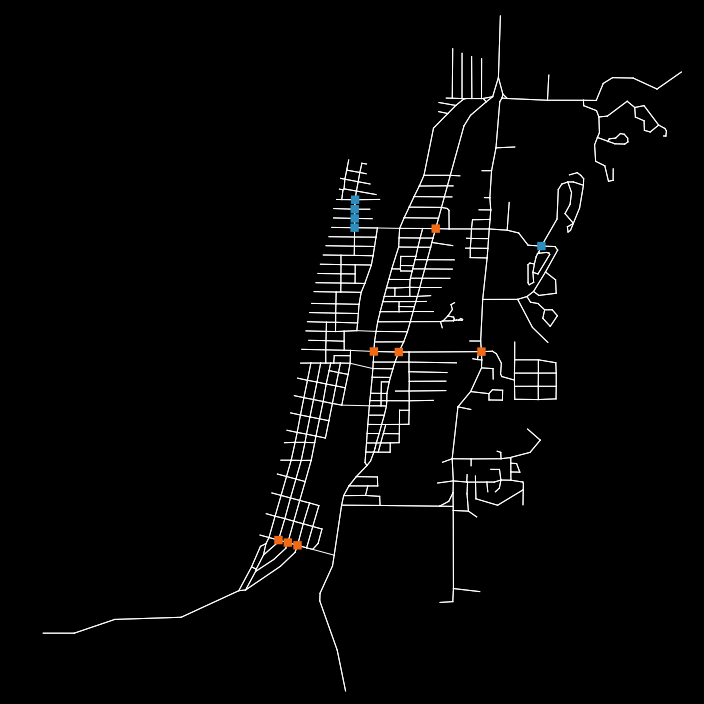
\includegraphics[width=\textwidth]{images/analisi/comparison-base-in-out-flow-25-75-car.png}
        \caption{25 pedoni 75 auto}
    \end{subfigure}
    \begin{subfigure}{0.475\textwidth}
        \centering
        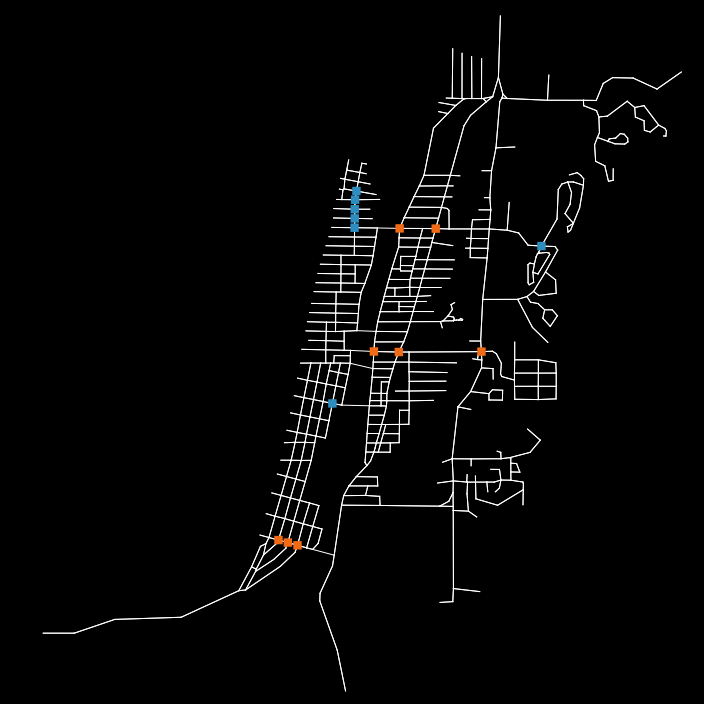
\includegraphics[width=\textwidth]{images/analisi/comparison-base-in-out-flow-0-100-car.png}
        \caption{0 pedoni 100 auto}
    \end{subfigure}
    \caption{}
    \label{fig:analisi-comparison-in-out-flow-map-base}
\end{figure}

\begin{figure}[ht]
    \centering
    \begin{subfigure}{0.475\textwidth}
        \centering
        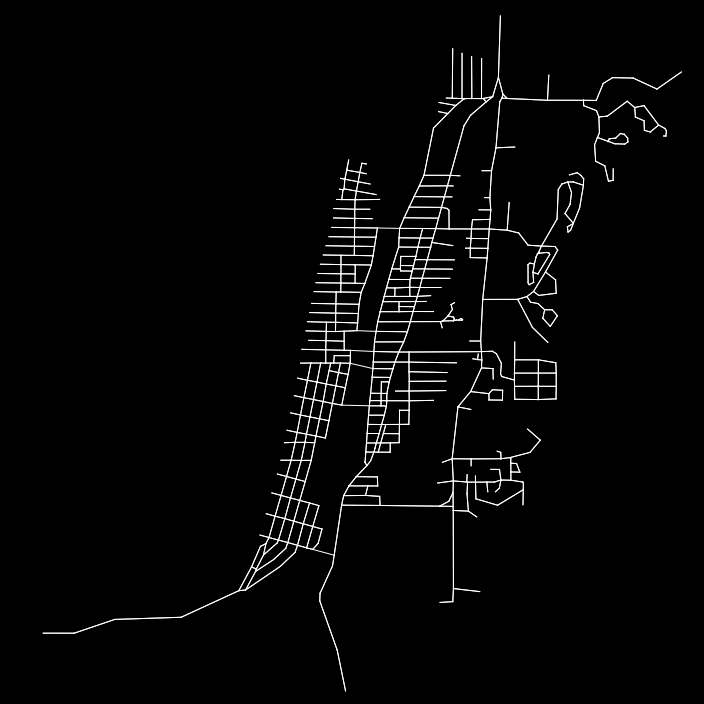
\includegraphics[width=\textwidth]{images/analisi/comparison-new-in-out-flow-75-25-car.png}
        \caption{75 pedoni 25 auto}
    \end{subfigure}
    \begin{subfigure}{0.475\textwidth}
        \centering
        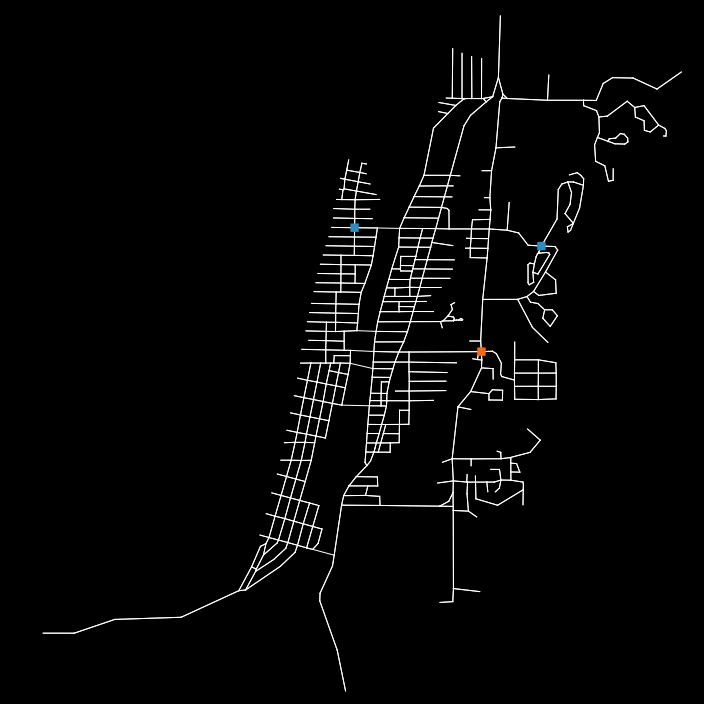
\includegraphics[width=\textwidth]{images/analisi/comparison-new-in-out-flow-50-50-car.png}
        \caption{50 pedoni 50 auto}
    \end{subfigure}
    \begin{subfigure}{0.475\textwidth}
        \centering
        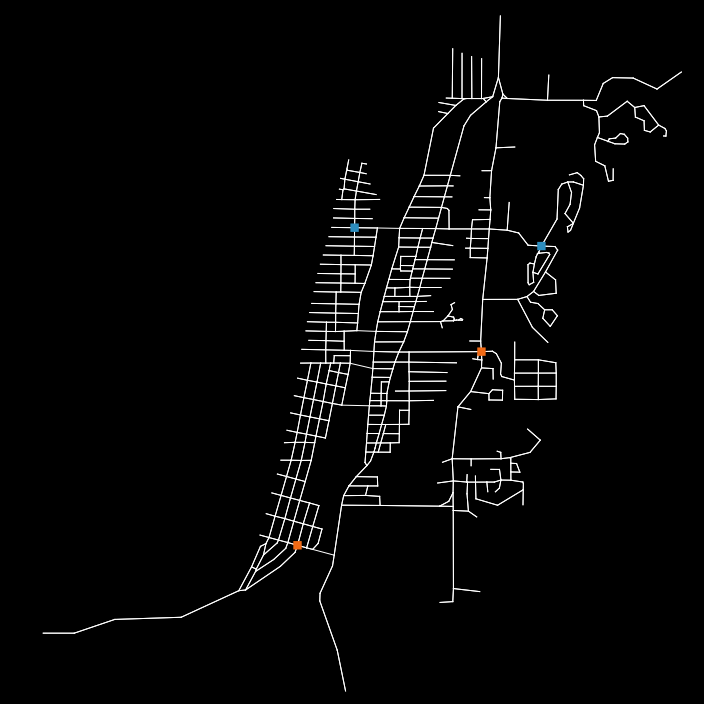
\includegraphics[width=\textwidth]{images/analisi/comparison-new-in-out-flow-25-75-car.png}
        \caption{25 pedoni 75 auto}
    \end{subfigure}
    \begin{subfigure}{0.475\textwidth}
        \centering
        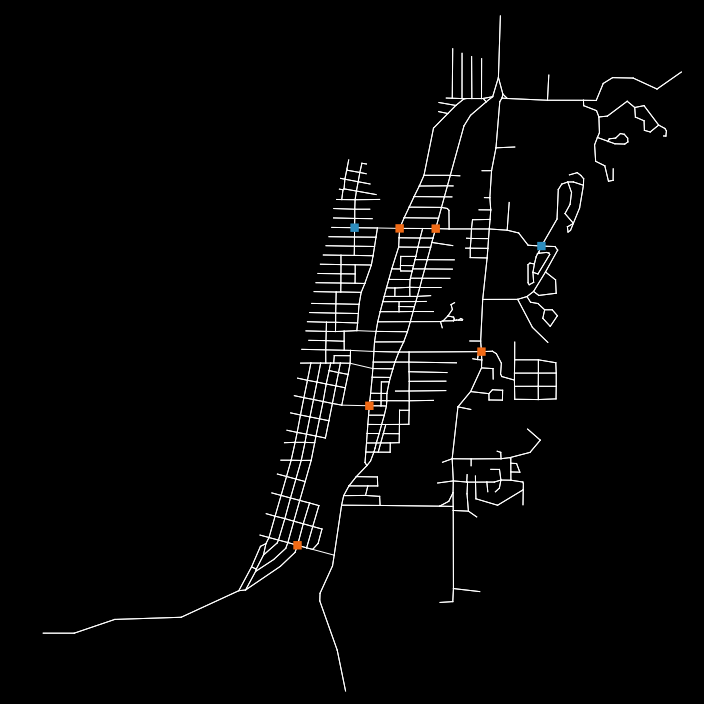
\includegraphics[width=\textwidth]{images/analisi/comparison-new-in-out-flow-0-100-car.png}
        \caption{0 pedoni 100 auto}
    \end{subfigure}
    \caption{}
    \label{fig:analisi-comparison-in-out-flow-map-new}
\end{figure}

\pagebreak

\subsubsection*{Tempi di attesa}
Infine per il modello esteso vengono analizzati i tempi di attesa nelle intersezioni per le auto,
ovvero il tempo che passa da quando un'auto arriva all'incrocio a quando ha il via libera. 
Inoltre i tempi sono distinti tra i due tipi di intersezione: AWSC e TWSC.

Come si può vedere nella tabella \ref{tab:analisi-car-delay}, con una percentuale più bassa di auto le intersezioni AWSC 
hanno in media tempi di attesa più lunghi mentre le intersezioni TWSC hanno tempi più brevi.

Per quanto riguarda le intersezioni TWSC, i tempi di attesa massimi sono più alti rispetto agli AWSC in tutti i casi a eccezione di quello con 25\% auto, 
per via della presenza degli stop nelle strade secondarie.

Nella figura \ref{fig:analisi-comparison-car-delay} vengono riportati i tempi di attesa al variare del numero di auto,
per ogni intersezione.

\begin{table}[ht]
    \centering
    \begin{tabular}{|c|c|c|c|c|c|}
    \hline
         & 25\% cars & 50\% cars & 75\% cars & 100\% cars & intersection \\ \hline
    mean & 34 s  & 32 s  & 29 s  & 24 s  & AWSC         \\ \hline
    max  & 267 s & 184 s & 202 s & 225 s & AWSC         \\ \hline
    mean & 8 s   & 13 s  & 18 s  & 31 s  & TWSC         \\ \hline
    max  & 142 s & 189 s & 237 s & 406 s & TWSC         \\ \hline
    \end{tabular}
    \caption{Confronto dei tempi di attesa massimi e medi per i due tipi di intersezioni al variare della percentuale di auto considerate.}
    \label{tab:analisi-car-delay}
\end{table}

\begin{figure}
    \centering
    \begin{subfigure}{0.475\textwidth}
        \centering
        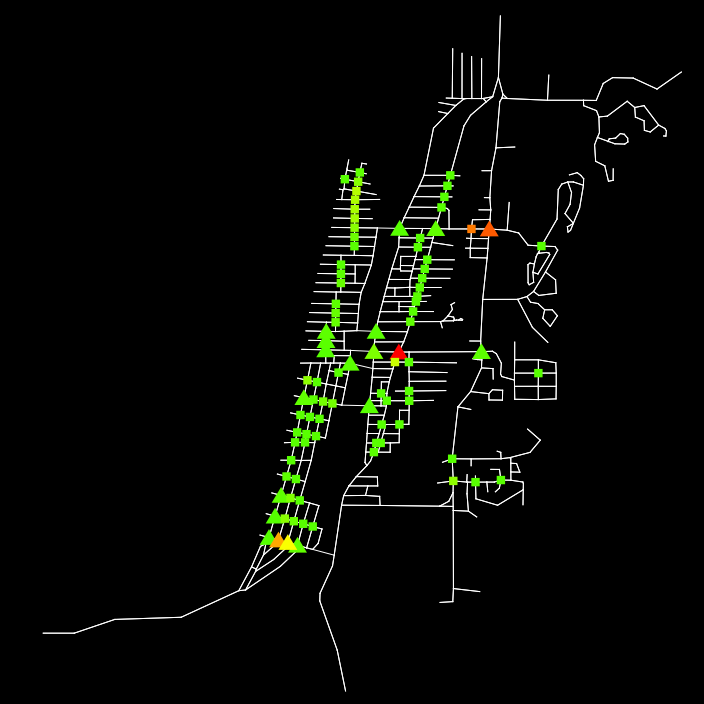
\includegraphics[width=\textwidth]{images/analisi/comparison-car-delay-75-25.png}
        \caption{75 pedoni 25 auto}
    \end{subfigure}
    \begin{subfigure}{0.475\textwidth}
        \centering
        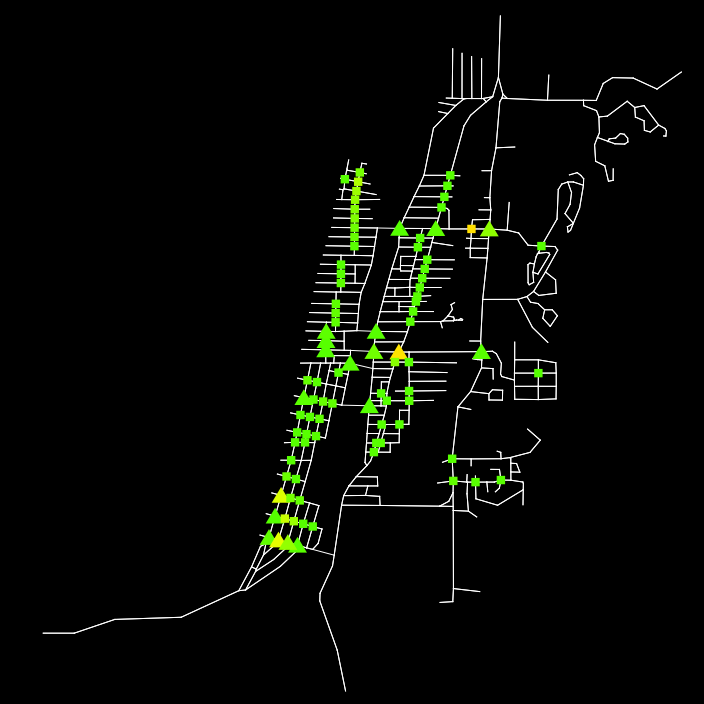
\includegraphics[width=\textwidth]{images/analisi/comparison-car-delay-50-50.png}
        \caption{50 pedoni 50 auto}
    \end{subfigure}

    \begin{subfigure}{0.475\textwidth}
        \centering
        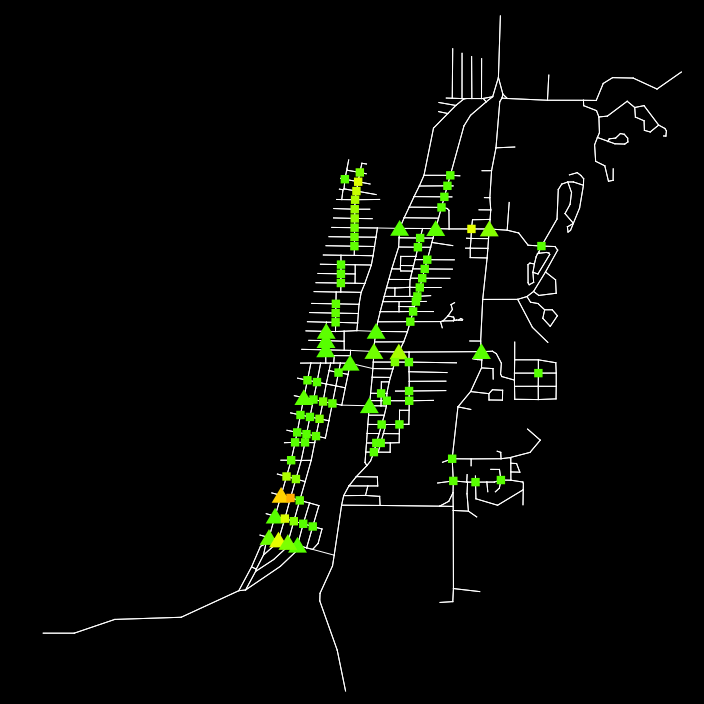
\includegraphics[width=\textwidth]{images/analisi/comparison-car-delay-25-75.png}
        \caption{25 pedoni 75 auto}
    \end{subfigure}
    \begin{subfigure}{0.475\textwidth}
        \centering
        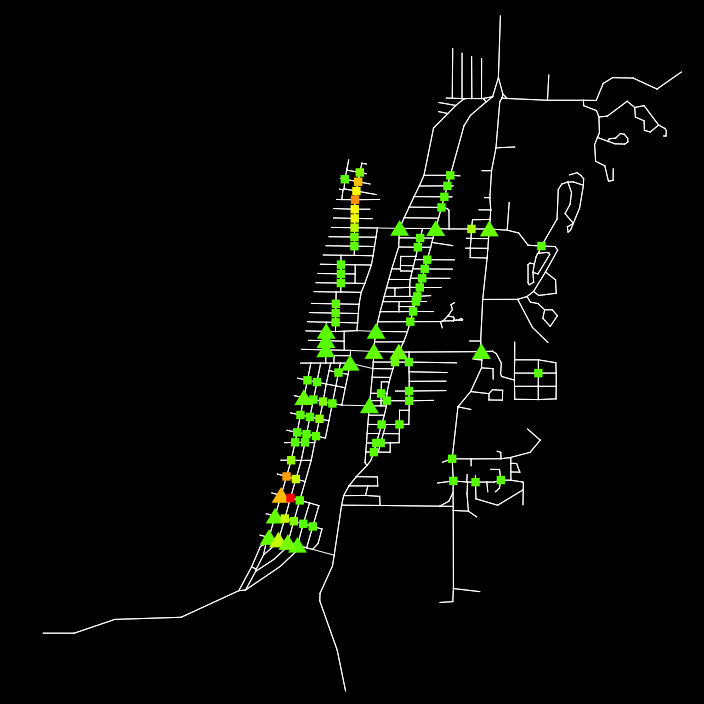
\includegraphics[width=\textwidth]{images/analisi/comparison-car-delay-0-100.png}
        \caption{0 pedoni 100 auto}
    \end{subfigure}
    \caption{tempo di attesa nelle intersezioni al variare della percentuale di auto considerata dove il colore rappresenta la lunghezza dei tempi di attesa, mentre i triangoli rappresentano gli AWSC ed i quadrati i TWSC.}
    \label{fig:analisi-comparison-car-delay}
\end{figure}

\subsection*{Comparazione Modello Base con Modello Wang 2021}
